%% arrowLength=10
%% linkWidth=3
%% input fy=50*node.pos
%% output fx=550
%% output fy=50*node.pos+25
%% MAX_FONT_SIZE=8
Imena razredov v glavah matrik zmot so okrajšana zaradi formatiranja dokumenta.
\begin{table}[H]
    \begin{center}
        \begin{tabular}{||l c c c||}
            \hline
            & 1        & 2        & 3 \\ [0.5ex]
            \hline
            velikost populacije               & 200      & 250      & 350      \\
            \hline
            največje število globokih vozlišč & 15       & 20       & 40       \\
            \hline
            največje število povezav          & 30       & 50       & 100      \\
            \hline
            največje število prečkanj         & 2        & 3        & 4        \\
            \hline
            delež mutiranih potomcev          & 10\%     & 10\%     & 10\%     \\
            \hline
            prispevek kompleksnosti           & -0.00001 & -0.00001 & -0.00001 \\
            \hline
            število generacij                 & 200      & 250      & 300      \\
            \hline
        \end{tabular}
    \end{center}
    \caption{Nabori inicializacijskih parametrov poganjanja na množici Shuttle.}
    \label{tab:param_statlog}
\end{table}

\subsection{Prvi nabor}\label{subsec:dodatek-statlog-prvi-nabor}
%% branch shuttle
%% 200 15 30 2 true 0.1 100 true -0.00001 200 ACC
\begin{table}[H]
    \begin{center}
        \begin{tabular}{|| c | c c || c c ||}
            \hline
            \multirow{2}{*}{št. zagona} & \multicolumn{2}{c||}{točnost najboljšega agenta} & \multicolumn{2}{c||}{MCC najboljšega agenta} \\ \cline{2-5}
            & učna   & testna          & učna  & testna                  \\
            \hline
            1        & 91.3\% & 91.8\%          & 0.656 & 0.658                   \\
            \hline
            2        & 86.2\% & 86.8\%          & 0.628 & 0.632                   \\
            \hline
            3        & 84.0\% & 84.7\%          & 0.753 & \textbf{0.760 (92.1\%)} \\
            \hline
            4        & 86.8\% & 87.4\%          & 0.572 & 0.578                   \\
            \hline
            5        & 91.8\% & \textbf{92.4\%} & 0.744 & 0.752                   \\
            \hline
            $\sigma$ & 0.030  & 0.030           & 0.069 & 0.070                   \\
            \hline
        \end{tabular}
    \end{center}
    \caption{Rezultat prvega nabora parametrov.}
    \label{tab:statlog_result_1}
\end{table}

\begin{table}[H]
    \centering
    \begin{tabular}{||rcccccccc||}
        \hline
        razred    & RF    & FC & FO & High & Bypass & BC & BO & vsota \\ \hline
        Rad Flow  & 11405 & 0  & 10 & 61   & 1      & 1  & 0  & 11478 \\ \hline
        Fpv Close & 8     & 0  & 0  & 5    & 0      & 0  & 0  & 13    \\ \hline
        Fpv Open  & 11    & 0  & 21 & 6    & 1      & 0  & 0  & 39    \\ \hline
        High      & 998   & 0  & 0  & 1157 & 0      & 0  & 0  & 2155  \\ \hline
        Bypass    & 0     & 0  & 0  & 0    & 808    & 1  & 0  & 809   \\ \hline
        Bpv Close & 1     & 0  & 0  & 1    & 2      & 0  & 0  & 4     \\ \hline
        Bpv Open  & 0     & 0  & 2  & 0    & 0      & 0  & 0  & 2     \\ \hline
        vsota     & 12423 & 0  & 33 & 1230 & 812    & 2  & 0  & 14500 \\ \hline
    \end{tabular}
    \caption{Matrika zmot najbolj točnega agenta prvega nabora. Agent lahko pravilno napove vse razrede razen \enquote{Fpv Close}, \enquote{Bpv Close} in \enquote{Bpv Open}.}
    \label{tab:statlog_acc_1}
\end{table}

\begin{table}[H]
    \centering
    \begin{tabular}{||rcccccccc||}
        \hline
        razred    & RF    & FC & FO & High & Bypass & BC & BO & vsota \\ \hline
        Rad Flow  & 11411 & 0  & 5  & 62   & 0      & 0  & 0  & 11478 \\ \hline
        Fpv Close & 3     & 0  & 0  & 10   & 0      & 0  & 0  & 13    \\ \hline
        Fpv Open  & 36    & 1  & 0  & 1    & 1      & 0  & 0  & 39    \\ \hline
        High      & 1024  & 0  & 0  & 1131 & 0      & 0  & 0  & 2155  \\ \hline
        Bypass    & 0     & 0  & 1  & 1    & 807    & 0  & 0  & 809   \\ \hline
        Bpv Close & 0     & 0  & 0  & 4    & 0      & 0  & 0  & 4     \\ \hline
        Bpv Open  & 2     & 0  & 0  & 0    & 0      & 0  & 0  & 2     \\ \hline
        vsota     & 12476 & 1  & 6  & 1209 & 808    & 0  & 0  & 14500 \\ \hline
    \end{tabular}
    \caption{Matrika zmot agenta z največjim MCC prvega nabora. Agent lahko pravilno napove razrede \enquote{Rad Flow}, \enquote{High} in \enquote{Bypass}.}
    \label{tab:statlog_mcc_1}
\end{table}

\begin{figure}[H]
    \begin{center}
        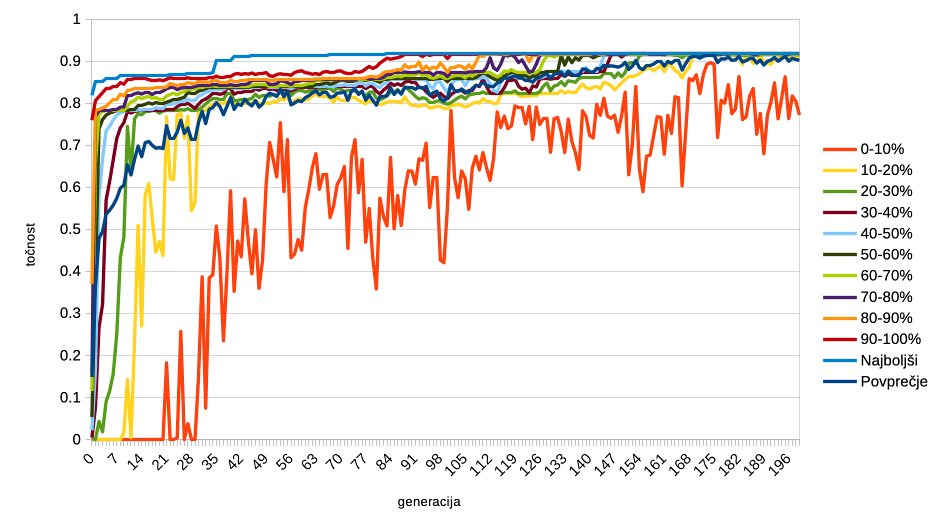
\includegraphics[width=13cm]{shuttle/1/acc}
    \end{center}
    \caption{Graf točnosti populacije najboljšega agenta prvega nabora skozi generacije.}
    \label{fig:statlog_acc_1}
\end{figure}

\begin{figure}[H]
    \begin{center}
        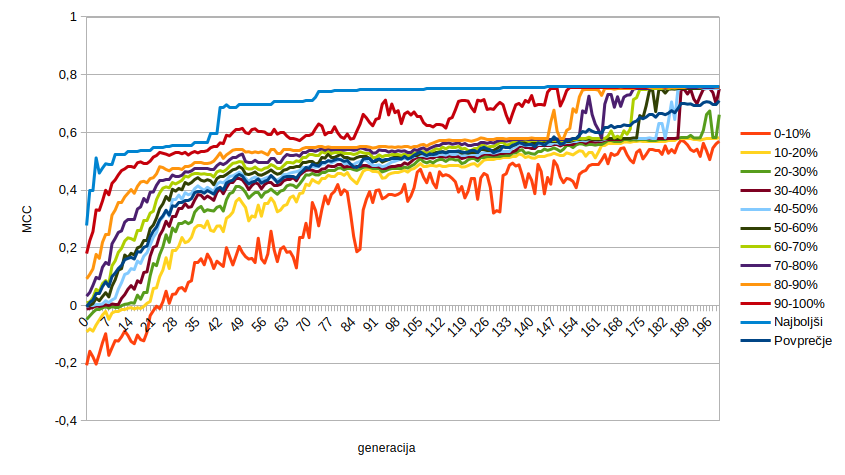
\includegraphics[width=13cm]{shuttle/1/mcc}
    \end{center}
    \caption{Graf MCC populacije najboljšega agenta prvega nabora skozi generacije.}
    \label{fig:statlog_mcc_1}
\end{figure}

\begin{figure}[H]
    \begin{center}
        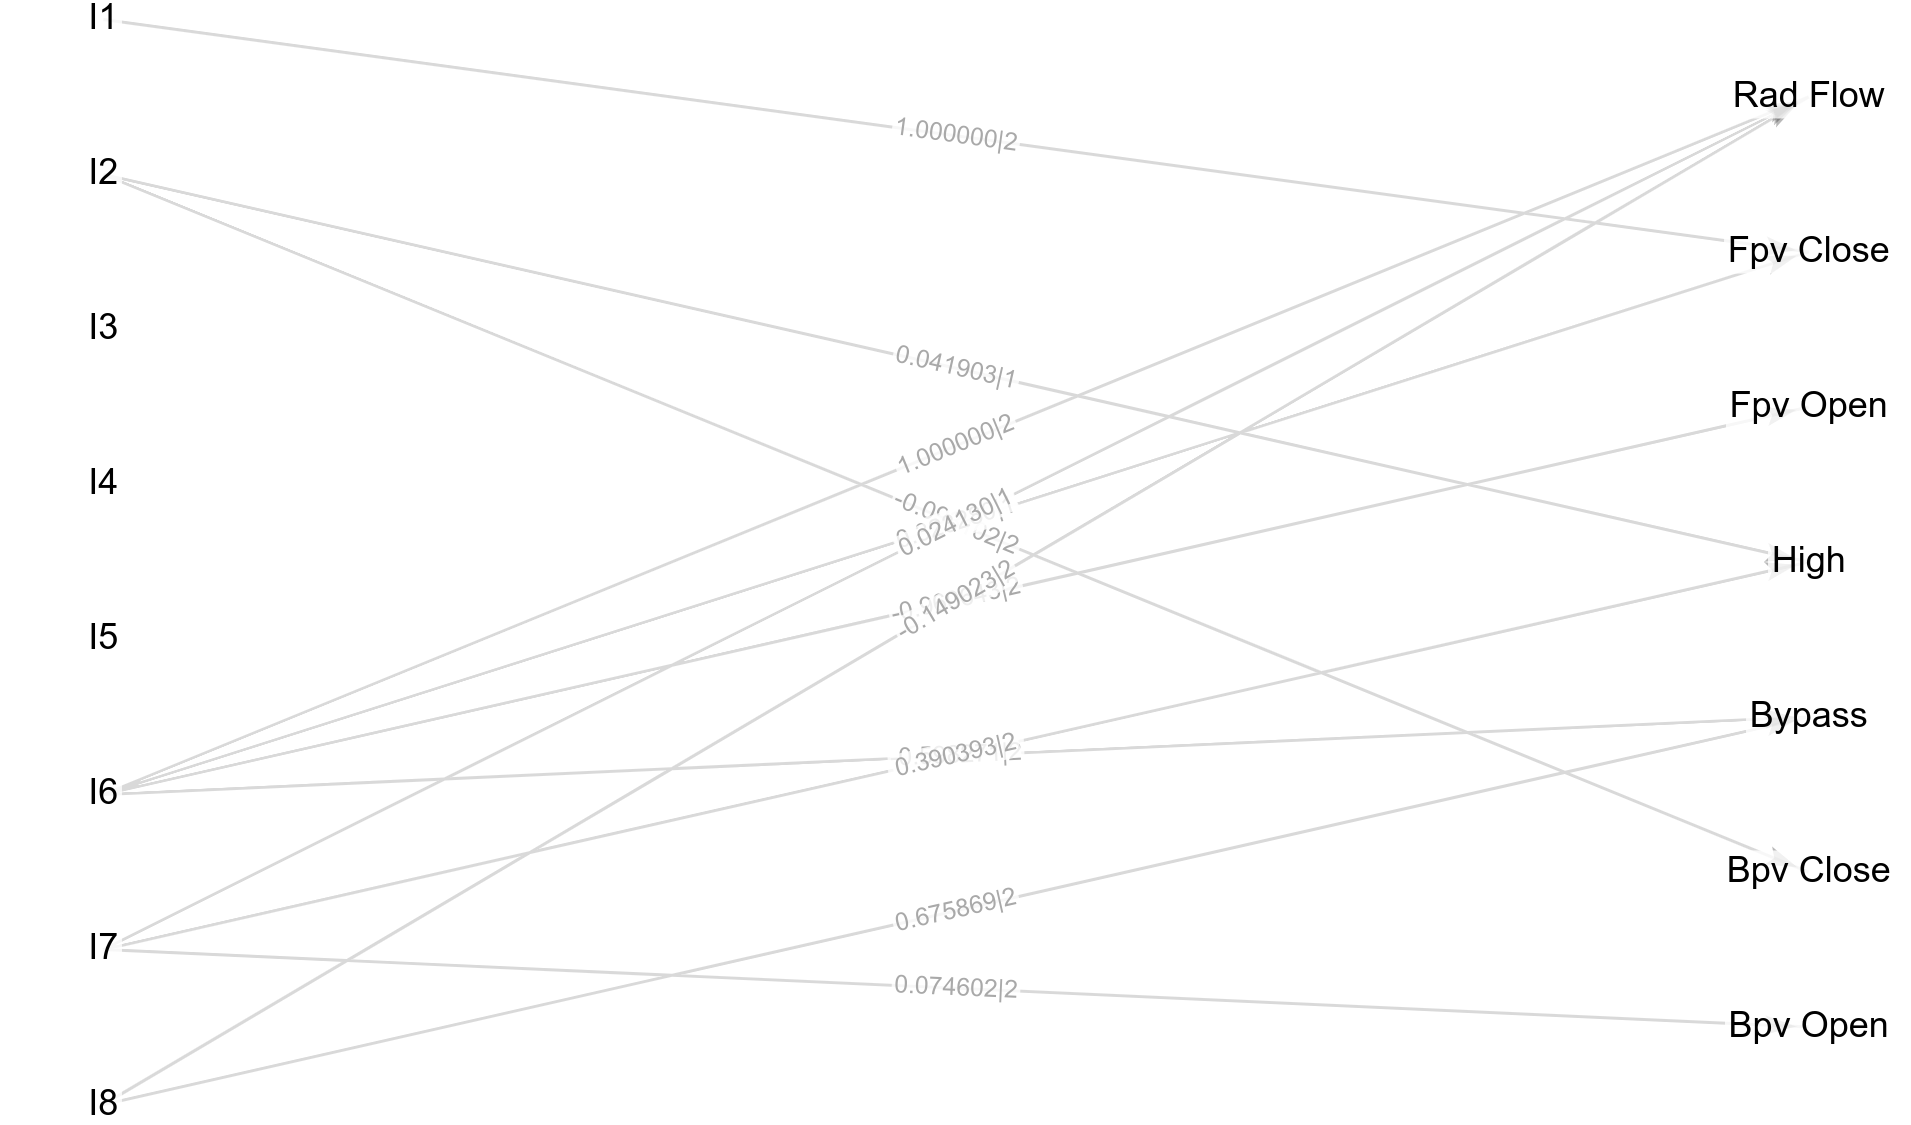
\includegraphics[width=13cm]{shuttle/1/acc_g}
    \end{center}
    \caption{Vizualizacija najbolj točnega agenta prvega nabora. Vsebuje 12 povezav.}
    \label{fig:statlog_acc_1_g}
\end{figure}

\begin{figure}[H]
    \begin{center}
        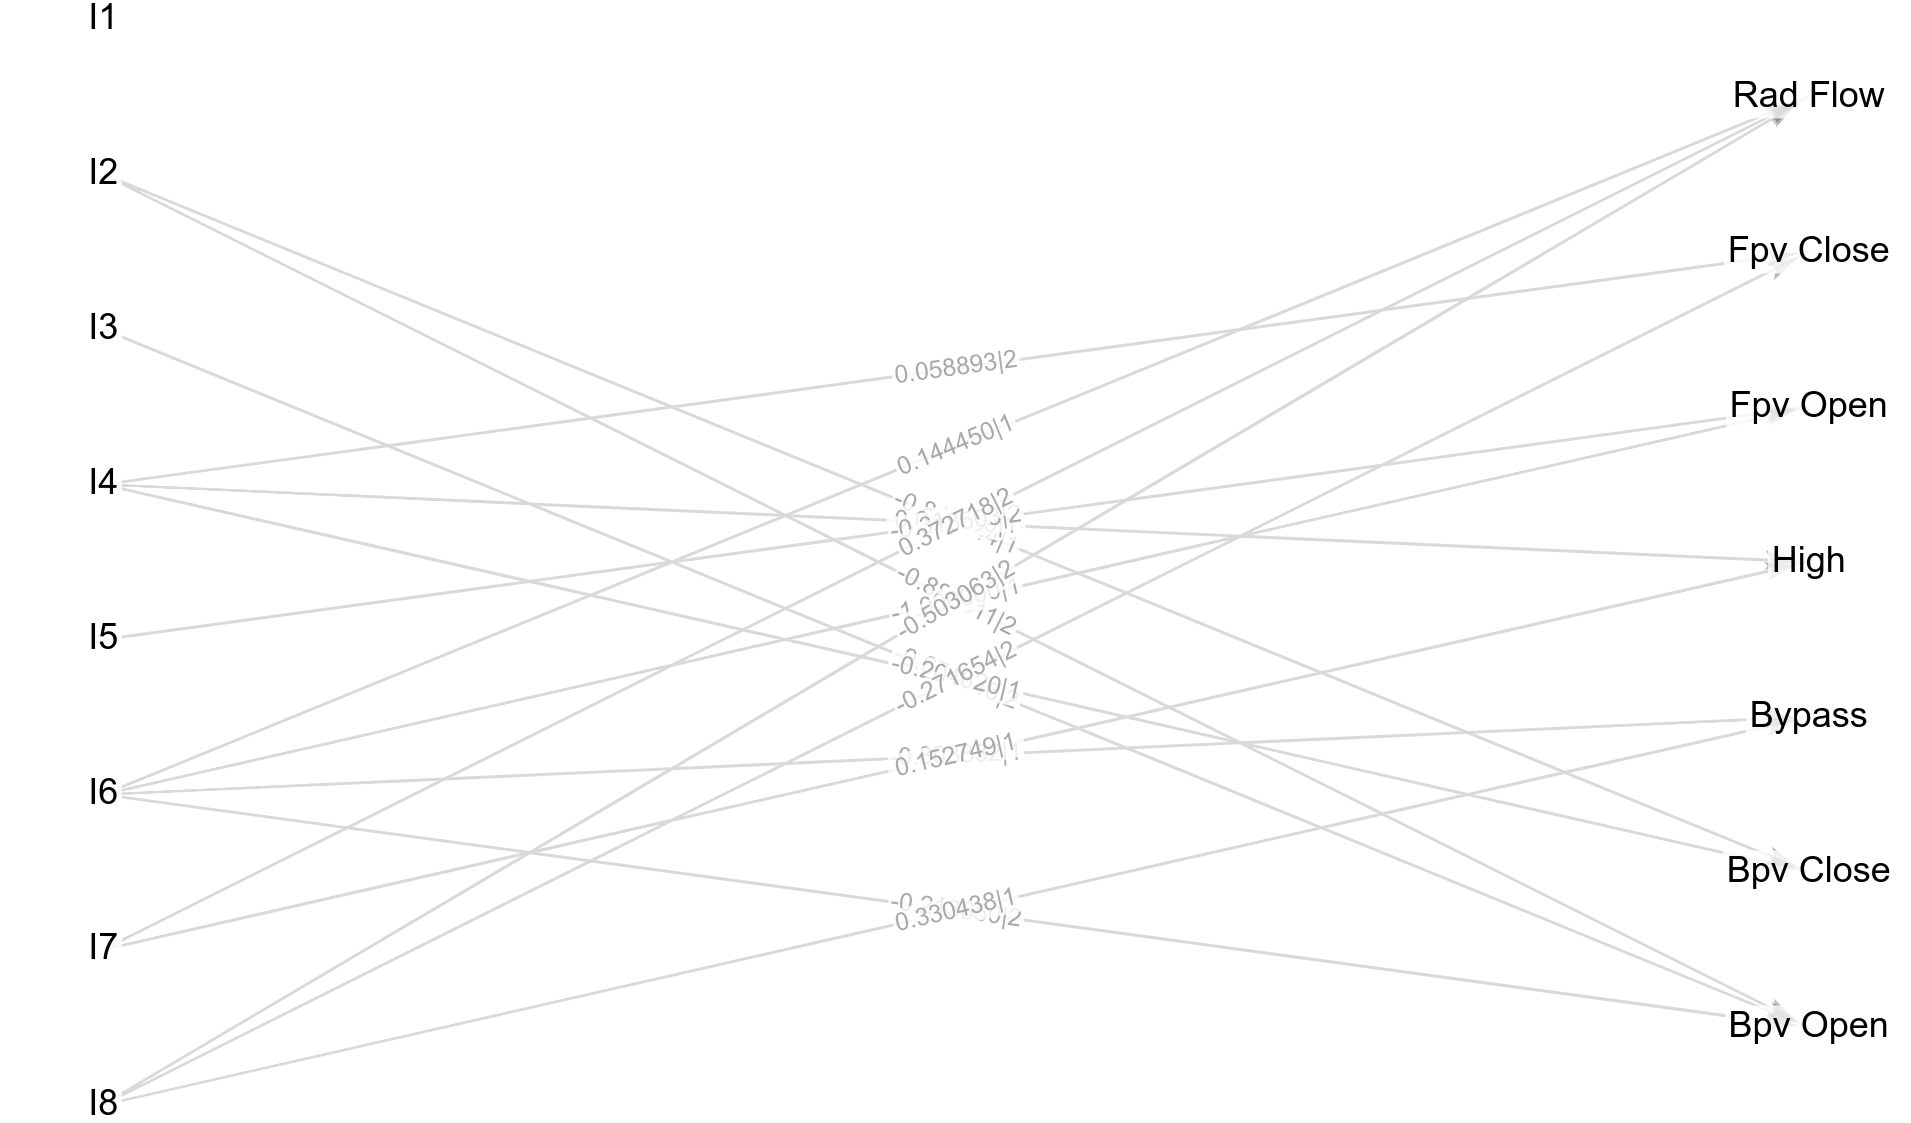
\includegraphics[width=13cm]{shuttle/1/mcc_g}
    \end{center}
    \caption{Vizualizacija agenta z največjim MCC prvega nabora. Vsebuje 1 globoko vozlišče in 21 povezav.}
    \label{fig:statlog_mcc_1_g}
\end{figure}

\subsection{Drugi nabor}\label{subsec:dodatek-statlog-drugi-nabor}
%% 250 20 50 3 true 0.1 125 true -0.00001 -0.00001 250 ACC
\begin{table}[H]
    \begin{center}
        \begin{tabular}{|| c | c c || c c ||}
            \hline
            \multirow{2}{*}{št. zagona} & \multicolumn{2}{c||}{točnost najboljšega agenta} & \multicolumn{2}{c||}{MCC najboljšega agenta} \\ \cline{2-5}
            & učna & testna       & učna & testna           \\
            \hline
            1        & 0\%  & 0\%          & 0    & 0                \\
            \hline
            2        & 0\%  & 0\%          & 0    & 0                \\
            \hline
            3        & 0\%  & 0\%          & 0    & \textbf{0 (0\%)} \\
            \hline
            4        & 0\%  & 0\%          & 0    & 0                \\
            \hline
            5        & 0\%  & \textbf{0\%} & 0    & 0                \\
            \hline
            $\sigma$ & 0    & 0            & 0    & 0                \\
            \hline
        \end{tabular}
    \end{center}
    \caption{Rezultat prvega nabora parametrov.}
    \label{tab:statlog_result_2}
\end{table}